% -*- mode: noweb; noweb-default-code-mode: R-mode; -*-
\documentclass[a4paper]{article}

\title{Product of Bivariate Copulas (PBC)}
\author{Pham Van Trung, Mazo Gildas}



\usepackage{a4wide}

\usepackage{Sweave}
\begin{document}



%\VignetteIndexEntry{PBC PBC}
\Sconcordance{concordance:PBC.tex:PBC.Rnw:%
1 10 1 1 0 13 1 1 2 4 0 2 2 4 0 2 2 4 0 2 2 4 0 1 2 2 1 2 2 4 1 1 2 1 0 %
3 1 12 0 2 2 1 0 1 1 3 0 1 3 4 0 1 2 1 1}


\maketitle

\section*{This document}
shows briefly how to use the \verb?PBC? package. See the package documentation and references for more informations. Please let the authors know about bugs or suggestions!

\section*{Let's get started}
Load the package.
\begin{Schunk}
\begin{Sinput}
> library(PBC)
\end{Sinput}
\end{Schunk}
Set the underlying graphical structure you wish, for instance
\begin{Schunk}
\begin{Sinput}
> g <- graph.formula(X1-X2, X2-X3, X3-X4, X4-X5, simplify = FALSE)
\end{Sinput}
\end{Schunk}
Pick a copula family (here Gumbel)
\begin{Schunk}
\begin{Sinput}
> myPBC <- pbcGumbel(g)
\end{Sinput}
\end{Schunk}
Or:
\begin{Schunk}
\begin{Sinput}
> myPBC <- pbc(g, model="gumbel") 
\end{Sinput}
\end{Schunk}
You can visualize the graph in Figure \ref{graph}.
\begin{figure}[htbp]
  \begin{center}
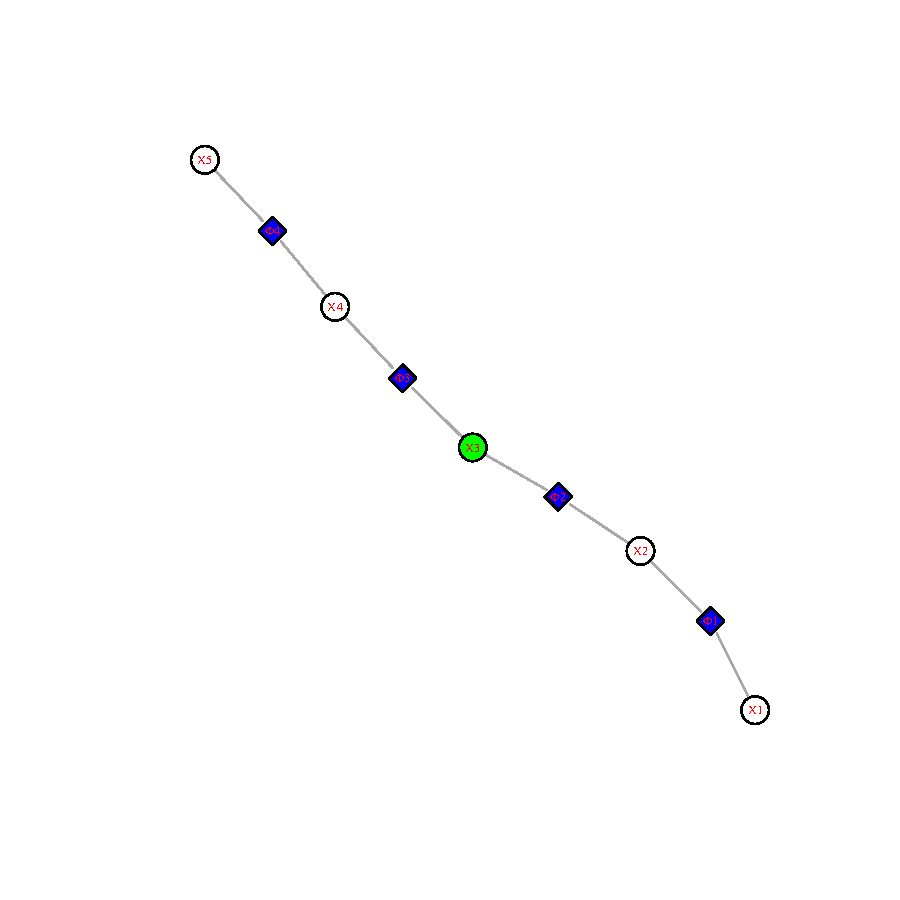
\includegraphics{PBC-005}
     \caption{Graph underlying the PBC model.}
     \label{graph}
  \end{center}
\end{figure}
Generate $n$ observations from that model with the parameter vector $\theta$.
\begin{Schunk}
\begin{Sinput}
> theta <- 1:4
> n <- 100
> data <- rPBC(n, theta, myPBC)
> head(data)
\end{Sinput}
\begin{Soutput}
          [,1]      [,2]      [,3]       [,4]      [,5]
[1,] 0.4207798 0.4129958 0.3961161 0.34178897 0.3904424
[2,] 0.5765883 0.4706939 0.4174468 0.39497048 0.7239168
[3,] 0.4576926 0.5401168 0.8620587 0.04900605 0.5249799
[4,] 0.4096496 0.9234606 0.9544151 0.07820935 0.1144382
[5,] 0.8578222 0.3694362 0.3692440 0.67192170 0.7021367
[6,] 0.7780032 0.7220907 0.4635803 0.35661046 0.4217583
\end{Soutput}
\end{Schunk}
Estimate the parameters:
\begin{Schunk}
\begin{Sinput}
> init <- 1/runif(4)
> theta.hat <- pbcOptim(init, data, myPBC, method = 'BFGS')
\end{Sinput}
\end{Schunk}
\begin{Schunk}
\begin{Soutput}
[1] 0.7854512 1.4776297 3.7307616 3.9968941
\end{Soutput}
\end{Schunk}
The value for \verb?init? was set randomly. It is best to provide a first guess, for instance by finding the pairwise maximum likelihood estimate (you don't need this package for that).
\end{document}
